\documentclass[conference]{IEEEtran}

\usepackage[utf8]{inputenc}
\usepackage[T1]{fontenc}
\usepackage{graphicx}
\usepackage{amsmath,amssymb}
\usepackage{booktabs}
\usepackage{multirow}
\usepackage{siunitx}
\usepackage{cite}
\usepackage{url}
\usepackage{balance}
\usepackage{hyperref}
\hypersetup{colorlinks=true, linkcolor=black, citecolor=black, urlcolor=black}
\usepackage{enumitem}

\title{Longitudinal Embedding Drift in Facial Representations: A Study of Temporal Stability and Verification Performance}

\author{
\IEEEauthorblockN{Harshinder Singh\IEEEauthorrefmark{1},\
Gyan Sharma\IEEEauthorrefmark{1},\
Devansh Goel\IEEEauthorrefmark{1},\
Siddhant Nirwal\IEEEauthorrefmark{1}}
\IEEEauthorblockA{\IEEEauthorrefmark{1}Department of Computer Science and Engineering\
ABES Institute of Technology\
Ghaziabad, India}
}

\begin{document}
\maketitle

\begin{abstract}
Face recognition systems typically evaluate whether two images belong to the same identity, but a different question is equally important: how stable is the numerical representation of the same person across longitudinal observations? We study this question using MORPH, a longitudinal face database, and fixed ArcFace-based embeddings. We construct an identity-disjoint train/validation/test protocol, measure embedding drift as $1 - \cos(\mathbf{e}_i, \mathbf{e}_j)$, and relate drift to genuine verification outcomes. In this MORPH cohort, the same-person face embedding was not perfectly stable across time, and higher observed drift was associated with larger longitudinal age gaps. Identity-level drift was heterogeneous, indicating that representation change is not uniform across individuals. Verification performance remained strong at the fixed operating threshold in the held-out test split, but failure rates increased markedly for larger age gaps and for high-drift comparisons. We interpret these findings as observational evidence about representation stability and verification behavior, not as causal proof of aging effects or a validated re-enrollment policy. The study motivates future drift-aware re-enrollment research while emphasizing that adaptive re-enrollment remains a direction for future experimental validation.
\end{abstract}

\begin{IEEEkeywords}
Face recognition, face embeddings, longitudinal analysis, embedding drift, ArcFace.
\end{IEEEkeywords}

\section{Introduction}
\label{sec:introduction}
Face recognition has become a mature research area, yet most evaluation protocols focus on matching two images at a single point in time or under controlled acquisition conditions. Longitudinal face data introduces a different problem: the same identity is observed repeatedly over time, and the face representation may drift as a function of age, acquisition conditions, and other covariates. This motivates a complementary question to the usual same-vs-different identity task: how stable is a person's face embedding across repeated observations, and how is that stability related to verification performance?

This paper studies this question in a longitudinal MORPH setting using fixed ArcFace embeddings. We distinguish between conventional recognition accuracy and representation stability. A face-recognition system may still perform well overall while the underlying representation of the same identity changes measurably over time. Our objective is therefore not to claim a universal aging mechanism or a new recognition algorithm, but to characterize longitudinal embedding drift and its relationship to genuine verification outcomes.

The research question is direct: How much does a person's face embedding change across longitudinal observations, how does this embedding drift vary across individuals and longitudinal age gaps, and how is representation drift related to face-verification performance? This distinction matters because it reframes the problem from a binary identity match question to a temporal stability question. The observed drift can be used to motivate adaptive re-enrollment, but adaptive re-enrollment itself is not experimentally validated here and remains future work.

The contributions of this study are as follows. First, we characterize longitudinal drift in a large MORPH cohort using fixed, identity-disjoint train/validation/test splits. Second, we quantify how observed drift changes across longitudinal age-gap groups. Third, we evaluate the relationship between drift and genuine verification performance under a frozen threshold. Fourth, we analyze identity-level heterogeneity in representative trajectories. Fifth, we report an exploratory individualized stability model, showing that the first Identity Stability Index formulation did not add predictive information beyond current drift. Together, these findings provide a cautious empirical basis for future drift-aware re-enrollment work rather than a validated re-enrollment policy.

\section{Related Work}
\label{sec:relatedwork}
Face recognition systems have been transformed by deep embedding models such as FaceNet~\cite{schroff2015facenet}, CosFace~\cite{wang2018cosface}, and ArcFace~\cite{deng2019arcface}. These methods learn embeddings such that semantically similar faces are represented by nearby vectors, while different identities are separated in feature space. ArcFace remains a strong reference model for fixed-feature evaluations because it provides a stable backbone widely used in face-recognition research.

Longitudinal face analysis is closely related to aging and template adaptation. MORPH is a classic longitudinal face dataset designed for age progression studies and repeated observations of the same identities over time~\cite{ricanek2006morph}. AgeDB is a widely used benchmark for age-invariant face recognition and age-gap evaluation~\cite{moschoglou2017agedb}. These datasets support analysis of how image appearance and model representations evolve as people age, but they do not fully isolate the causal effects of biological age from changes in lighting, pose, expression, camera, and image acquisition.

A substantial body of recognition work investigates how elapsed time and age progression affect matching performance, including studies of age-invariant recognition and template aging~\cite{park2010age,han2013age}. However, much of this literature focuses on same-vs-different identity decisions rather than the representational drift of the same identity itself. Our work is intentionally different: instead of asking only whether two images match, we quantify the amount of change in the embedding of the same person over time and ask whether larger observed drift corresponds to increased verification failure.

This distinction is critical. The observed relationship between drift and failure is statistical and empirical; it does not establish causality, and it does not yet justify a validated adaptive re-enrollment system. In this sense, our study contributes to a longitudinal representation-stability perspective rather than a direct application-oriented recognition system.

\section{Dataset and Experimental Protocol}
\label{sec:dataset}
\subsection{Dataset audit and selection}
We used MORPH as the primary longitudinal dataset because it contains repeated observations of the same identities across recorded ages, making it suitable for studying within-identity representation change over time. The project audit identified approximately 50,015 raw MORPH images and approximately 19,033 identities. The age variable used for modeling and ordering was the filename-derived age, which is an available longitudinal/acquisition variable but not a perfect biological-age measurement. This distinction is important: the age labels are useful for ordering and age-gap analysis, but they should not be interpreted as exact physical age or a causal treatment of aging.

AgeDB was also audited as a secondary dataset. It contains approximately 12,240 images from about 440 identities with four protocol files for 5-year, 10-year, 20-year, and 30-year splits, each with about 6,000 records and roughly 3,000 genuine and 3,000 impostor comparisons. During image-level reconstruction, 15,716 records were ambiguous or unresolved. We therefore did not use AgeDB as the primary image-level embedding validation dataset for the main longitudinal MORPH study. It is noted here briefly because it supports the broader literature context and the project audit, but it was not the main evidence source for the claims in this paper.

\subsection{Identity-disjoint research split}
The original MORPH dataset was not organized for an identity-disjoint longitudinal evaluation objective. To reduce identity leakage and to provide a cleaner longitudinal analysis, we constructed a research split at random seed 42. The resulting split was identity-disjoint across train, validation, and test partitions.

\begin{table}[t]
\centering
\caption{Dataset summary.}
\label{tab:dataset}
\begin{tabular}{@{}lrr@{}}
\toprule
Dataset property & Value & Notes \\
\midrule
MORPH raw images & 50,015 & Primary longitudinal dataset \\
MORPH successfully processed & 50,013 & 2 failed cases \\
MORPH identities (raw audit) & 19,033 & Approximate audit count \\
AgeDB images & 12,240 & Secondary audit dataset \\
AgeDB identities & 440 & Approximate audit count \\
AgeDB protocol files & 4 & 5-, 10-, 20-, 30-year \\
Eligible MORPH longitudinal pairs & 84,133 & Same identity, different observation \\
\bottomrule
\end{tabular}
\end{table}

\begin{table}[t]
\centering
\caption{Identity-disjoint research split.}
\label{tab:split}
\begin{tabular}{@{}lrrrr@{}}
\toprule
Split & Identities & Images & Longitudinal pairs & Notes \\
\midrule
Train & 13,323 & 35,040 & 59,545 & No identity overlap \\
Validation & 2,855 & 7,581 & 12,303 & No identity overlap \\
Test & 2,855 & 7,394 & 12,289 & No identity overlap \\
\bottomrule
\end{tabular}
\end{table}

The final research split contained 13,323 train identities, 2,855 validation identities, and 2,855 test identities with no identity appearing across splits. This design was chosen to reduce identity leakage and to provide a more reliable evaluation of longitudinal drift in a held-out setting.

\subsection{Longitudinal pair construction}
After preprocessing, the project produced 84,133 eligible same-identity longitudinal pairs. A pair was defined as two different observations of the same identity with an age gap computed as the absolute difference in filename-derived age. The analytical reference was the youngest observation by filename-derived age, with filename tie-breaking as a deterministic ordering rule. This analytical reference is not necessarily a true enrollment image; it is an analytical baseline used to study longitudinal changes in a fixed representation space.

The longitudinal coverage was substantial: 13,119 identities had at least two observations, 7,514 had at least three, 3,872 had at least four, and 2,188 had at least five. Longer-span subsets were also present, including 326 identities with at least three observations spanning at least five years, 145 spanning at least ten years, and 26 spanning at least twenty years.

\section{Methodology}
\label{sec:methodology}
\subsection{Preprocessing and embedding extraction}
Raw MORPH images were processed with InsightFace face detection and ArcFace-compatible alignment using the standard $112 \times 112$ crop procedure. The preprocessing stage handled 50,013 of 50,015 raw images successfully, with 2 failures: \texttt{138612\_3F55.JPG} and \texttt{45148\_00M40.JPG}. Detection outcomes were 2 zero-face cases, 50,013 single-face cases, and 0 multiple-face cases. The aligned output was stored as BGR uint8; model normalization was deferred to the embedding-extraction stage.

We used InsightFace with the \texttt{buffalo\_l} model and extracted 512-dimensional ArcFace embeddings. We then applied L2 normalization. Quality checks confirmed 50,013 successful embeddings, 0 extraction failures, 0 missing embeddings, 0 unexpected embeddings, and all embeddings were finite, 512-dimensional, and approximately unit-normalized. The L2 norm statistics were tightly clustered around 1.0, with minimum 0.999999880791, maximum 1.000000119209, mean 0.999999982679, standard deviation approximately $3.19 \times 10^{-8}$, and maximum absolute deviation from 1.0 approximately $1.19 \times 10^{-7}$. Repeated inference produced zero difference and cosine similarity of exactly 1.0 in repeated checks.

\subsection{Drift definition}
For normalized embeddings $\mathbf{e}_i$ and $\mathbf{e}_j$, we define cosine similarity as
\begin{equation}
\text{sim}(\mathbf{e}_i, \mathbf{e}_j) = \frac{\mathbf{e}_i^T \mathbf{e}_j}{\lVert \mathbf{e}_i \rVert \lVert \mathbf{e}_j \rVert}
\end{equation}
with normalized embeddings, and embedding drift as
\begin{equation}
\text{drift} = 1 - \text{sim}(\mathbf{e}_i, \mathbf{e}_j).
\end{equation}
Here, low drift indicates a more similar representation and high drift indicates larger representation change. Euclidean distance was retained as a secondary consistency metric, but the primary metric is cosine-based drift. We do not interpret drift itself as recognition error; it is a representation change metric.

\subsection{Identity-level and age-gap analyses}
We computed identity-level drift summaries across all available same-identity longitudinal pairs. The identity-level distribution showed substantial heterogeneity, which is relevant because some identities changed more than others even under the same model and dataset. We also grouped observations by age gap: 0--2, 3--4, 5--9, 10--19, and 20+. This analysis was descriptive and observational. We do not claim that age alone causes embedding drift; instead, we report that observed drift increased with longitudinal age gap in the evaluated MORPH data, while multiple factors such as age, pose, illumination, expression, image quality, and device/acquisition conditions may contribute.

\subsection{Verification protocol}
For verification, we used genuine longitudinal comparisons and a deterministic within-split impostor set constructed with random seed 42. The primary threshold was selected on the validation split using the empirical 1\% impostor FAR rule and then frozen before testing. The selected similarity threshold was 0.206770330667, corresponding to a drift boundary of 0.793229669333. This operating threshold should be interpreted as a verification boundary, not as a validated adaptive re-enrollment threshold.

\section{Results}
\label{sec:results}
\subsection{Identity-level drift}
The identity-level summary across 13,119 identities was as follows: mean drift 0.2296, standard deviation 0.0813, median 0.2180, minimum 0.0559, maximum 1.2184, P25 0.1818, P75 0.2620, P90 0.3118, P95 0.3469, and P99 0.4653. These values show that representation change is not negligible even for the same identity and that there is substantial between-identity heterogeneity. The distribution is visualized in Fig.~\ref{fig:identity_drift_distribution}.

\subsection{Age-gap drift}
We observed increased mean drift with larger age gaps. For the MORPH pairs analyzed here, mean drift was approximately 0.236 for 0--2 years, 0.261 for 3--4 years, 0.305 for 5--9 years, 0.375 for 10--19 years, and 0.774 for 20+ years. The age-gap effect is shown in Fig.~\ref{fig:age_gap_drift}. This relationship was observational and consistent with the idea that larger temporal separation coincided with larger representation change in the evaluated dataset. It should not be read as a causal finding, because longitudinal comparisons confound age with acquisition conditions, pose, illumination, expression, and image quality.

\subsection{Verification performance}
The held-out test result remained strong at the frozen verification threshold. The test split achieved ROC-AUC 0.996201, EER 0.003745, FAR 0.008592, and FRR 0.007270. The validation and train performance were comparably strong (Table~\ref{tab:verification-performance}). These metrics indicate that despite measurable representation drift, the fixed ArcFace embedding and verification threshold remained highly discriminative overall in the evaluated MORPH sample.

\begin{table}[t]
\centering
\caption{Embedding and verification performance.}
\label{tab:verification-performance}
\begin{tabular}{@{}lrrrr@{}}
\toprule
Split & ROC-AUC & EER & FAR & FRR \\
\midrule
Train & 0.996767 & 0.002625 & 0.007598 & 0.005250 \\
Validation & 0.996745 & 0.002751 & 0.010157 & 0.005501 \\
Test & 0.996201 & 0.003745 & 0.008592 & 0.007270 \\
\bottomrule
\end{tabular}
\end{table}

\subsection{Age-gap verification failure}
At the test threshold, verification failure increased with age gap. The test-set FRR was 0.07\% for 0--2 years, 0.24\% for 3--4 years, 6.39\% for 5--9 years, 11.24\% for 10--19 years, and 61.29\% for 20+ years. The total pair counts were 11,114, 836, 219, 89, and 31, respectively. The 20+ group is small and should not be interpreted as a general population estimate; it represents a very limited sample in this dataset. The age-gap failure pattern is summarized in Table~\ref{tab:agegap} and Fig.~\ref{fig:age_gap_verification}.

\begin{table}[t]
\centering
\caption{Age-gap drift and verification performance on the test split.}
\label{tab:agegap}
\begin{tabular}{@{}lrrrr@{}}
\toprule
Age gap & Pairs & Mean drift & Acceptance & FRR \\
\midrule
0--2 & 11,114 & 0.2382 & 99.93\% & 0.07\% \\
3--4 & 836 & 0.2693 & 99.76\% & 0.24\% \\
5--9 & 219 & 0.3363 & 93.61\% & 6.39\% \\
10--19 & 89 & 0.3662 & 88.76\% & 11.24\% \\
20+ & 31 & 0.6681 & 38.71\% & 61.29\% \\
\bottomrule
\end{tabular}
\end{table}

\subsection{Drift bins and operating boundary}
The drift-bin analysis showed a consistent pattern: moderate drift values were still compatible with positive verification decisions, whereas sufficiently large drift values crossed the fixed verification operating boundary. For example, on the test split, 0.00--0.10, 0.10--0.20, 0.20--0.30, 0.30--0.40, 0.40--0.50, and 0.50--0.60 drift bins all had 100\% acceptance, while 0.80--0.90, 0.90--1.00, and $>1.00$ bins had 0\% acceptance. This illustrates that moderate drift can remain compatible with successful verification under a fixed operating threshold, whereas high drift can move comparisons outside the validated verification region. The threshold at 0.7932 is shown in Fig.~\ref{fig:boundary} and is interpreted as a verification boundary, not as a validated re-enrollment threshold.

\subsection{Longitudinal trajectories}
The trajectory analysis showed heterogeneous identity-specific patterns. Some identities had relatively stable drift behavior across repeated observations, others showed increasing drift with age, and some had nonlinear or irregular movement. Candidate return/persistent events were identified using a training-derived exploratory threshold of 0.361454629, but these are descriptive candidate events only and not evidence of a physiological mechanism or a production rule. Representative trajectories are shown in Fig.~\ref{fig:trajectories}. The identity-level heterogeneity suggests that the same dataset can contain both stable and unstable representation trajectories.

\section{Discussion}
\label{sec:discussion}
The main empirical result is not that embedding drift is a universal failure mode, but that it is measurable and varies with longitudinal separation. In the evaluated MORPH data, drift increased with larger age gaps, and larger age gaps were associated with higher FRR. The effect is not uniform across identities: the distribution of identity-level mean drift was broad, and some identities remained stable while others accumulated larger representation changes over time.

This pattern matters because it clarifies the distinction between representation stability and recognition success. A fixed recognition model can remain highly accurate overall even when substantial drift is present in some observations. In other words, the fixed ArcFace representation is not perfectly static across time, but the decision boundary remains strong enough to preserve high performance in many observed cases. This is consistent with our results: strong overall ROC-AUC and low EER, alongside increasing FRR at larger age gaps and high drift.

The data also show that high drift does not automatically imply verification failure; moderate drift can still be compatible with successful matching under a fixed threshold. This is why the boundary analysis should be interpreted carefully: the drift threshold is a convenient behavioral characterization in drift space, not a validated re-enrollment trigger. Such a threshold may help motivate future adaptive re-enrollment work, but it is not proof of a correct or optimal re-enrollment policy.

\section{Exploratory Identity Stability Index}
\label{sec:isi}
We also evaluated an exploratory individualized Identity Stability Index (ISI). This index used current reference drift and a small set of identity-specific historical terms, including historical percentile, historical z-score, median deviation, consecutive drift, and recent slope. The formulation was intended to estimate whether an identity's own historical behavior added information beyond current drift alone.

The final observed result was negative for the first formulation: the corrected production artifact showed that the ISI score had ROC-AUC 0.661054 and PR-AUC 0.367662, exactly matching the current reference drift baseline. The correlation between current drift and the ISI was 1.0. Therefore, in this dataset and with this implementation, the ISI did not demonstrate independent predictive value beyond current drift. This is an exploratory negative result and should be interpreted as methodological evidence against over-claiming individualized predictive power from the first ISI formulation.

\begin{table}[t]
\centering
\caption{Exploratory ISI comparison.}
\label{tab:isi}
\begin{tabular}{@{}lrrr@{}}
\toprule
Model & ROC-AUC & PR-AUC & Brier \\
\midrule
Current reference drift & 0.661054 & 0.367662 & 0.037012 \\
ISI & 0.661054 & 0.367662 & 0.037012 \\
\bottomrule
\end{tabular}
\end{table}

\section{Limitations}
\label{sec:limitations}
This study has several important limitations. First, MORPH is observational; the data capture repeated observations but not controlled longitudinal interventions. We therefore cannot infer a causal effect of age on embedding drift. Second, the age variable is filename-derived and is not a perfect biological-age measurement. Third, the observed drift may reflect multiple factors in addition to age, including illumination, pose, expression, facial hair, image quality, camera/device, compression, and appearance changes. Fourth, the 20+ year age-gap group contains only 31 test pairs, so estimates there are unstable and should be interpreted cautiously. Fifth, the fixed ArcFace model is pretrained and not re-optimized for this longitudinal setting. Sixth, the first ISI formulation was exploratory and did not add independent predictive value. Seventh, the Stage 8 bootstrap methodology was declared, but the executed analysis did not perform the intended bootstrap, so confidence intervals for the ISI analysis should not be claimed. Eighth, AgeDB was audited for supplemental context but was not used as the main image-level longitudinal validation set because image-level mapping remained ambiguous or unresolved. Ninth, any re-enrollment policy remains speculative and future work is required before any adaptive re-enrollment system can be considered validated.

\section{Conclusion and Future Work}
\label{sec:conclusion}
This paper provides an empirical characterization of longitudinal embedding drift in a large MORPH cohort. We observed that the same person's representation was not perfectly stable across repeated observations, that drift was heterogeneous across identities, and that larger longitudinal age gaps were associated with higher observed drift and lower verification acceptance in the evaluated sample. At the fixed verification threshold, the held-out test performance remained strong overall, but long-term separations exhibited substantially greater verification failure rates.

These findings support a temporal stability interpretation rather than a causal or policy claim. They motivate future work on drift-aware re-enrollment, but do not validate an adaptive re-enrollment algorithm. A robust future program would examine genuinely independent individualized stability models, identity-cluster bootstrap uncertainty, and policy simulations comparing no re-enrollment, fixed-period re-enrollment, drift-triggered re-enrollment, and individualized re-enrollment. Such studies should measure future FRR, number of template updates, unnecessary updates, and the trade-off between recognition stability and update frequency.

\begin{figure*}[t]
\centering
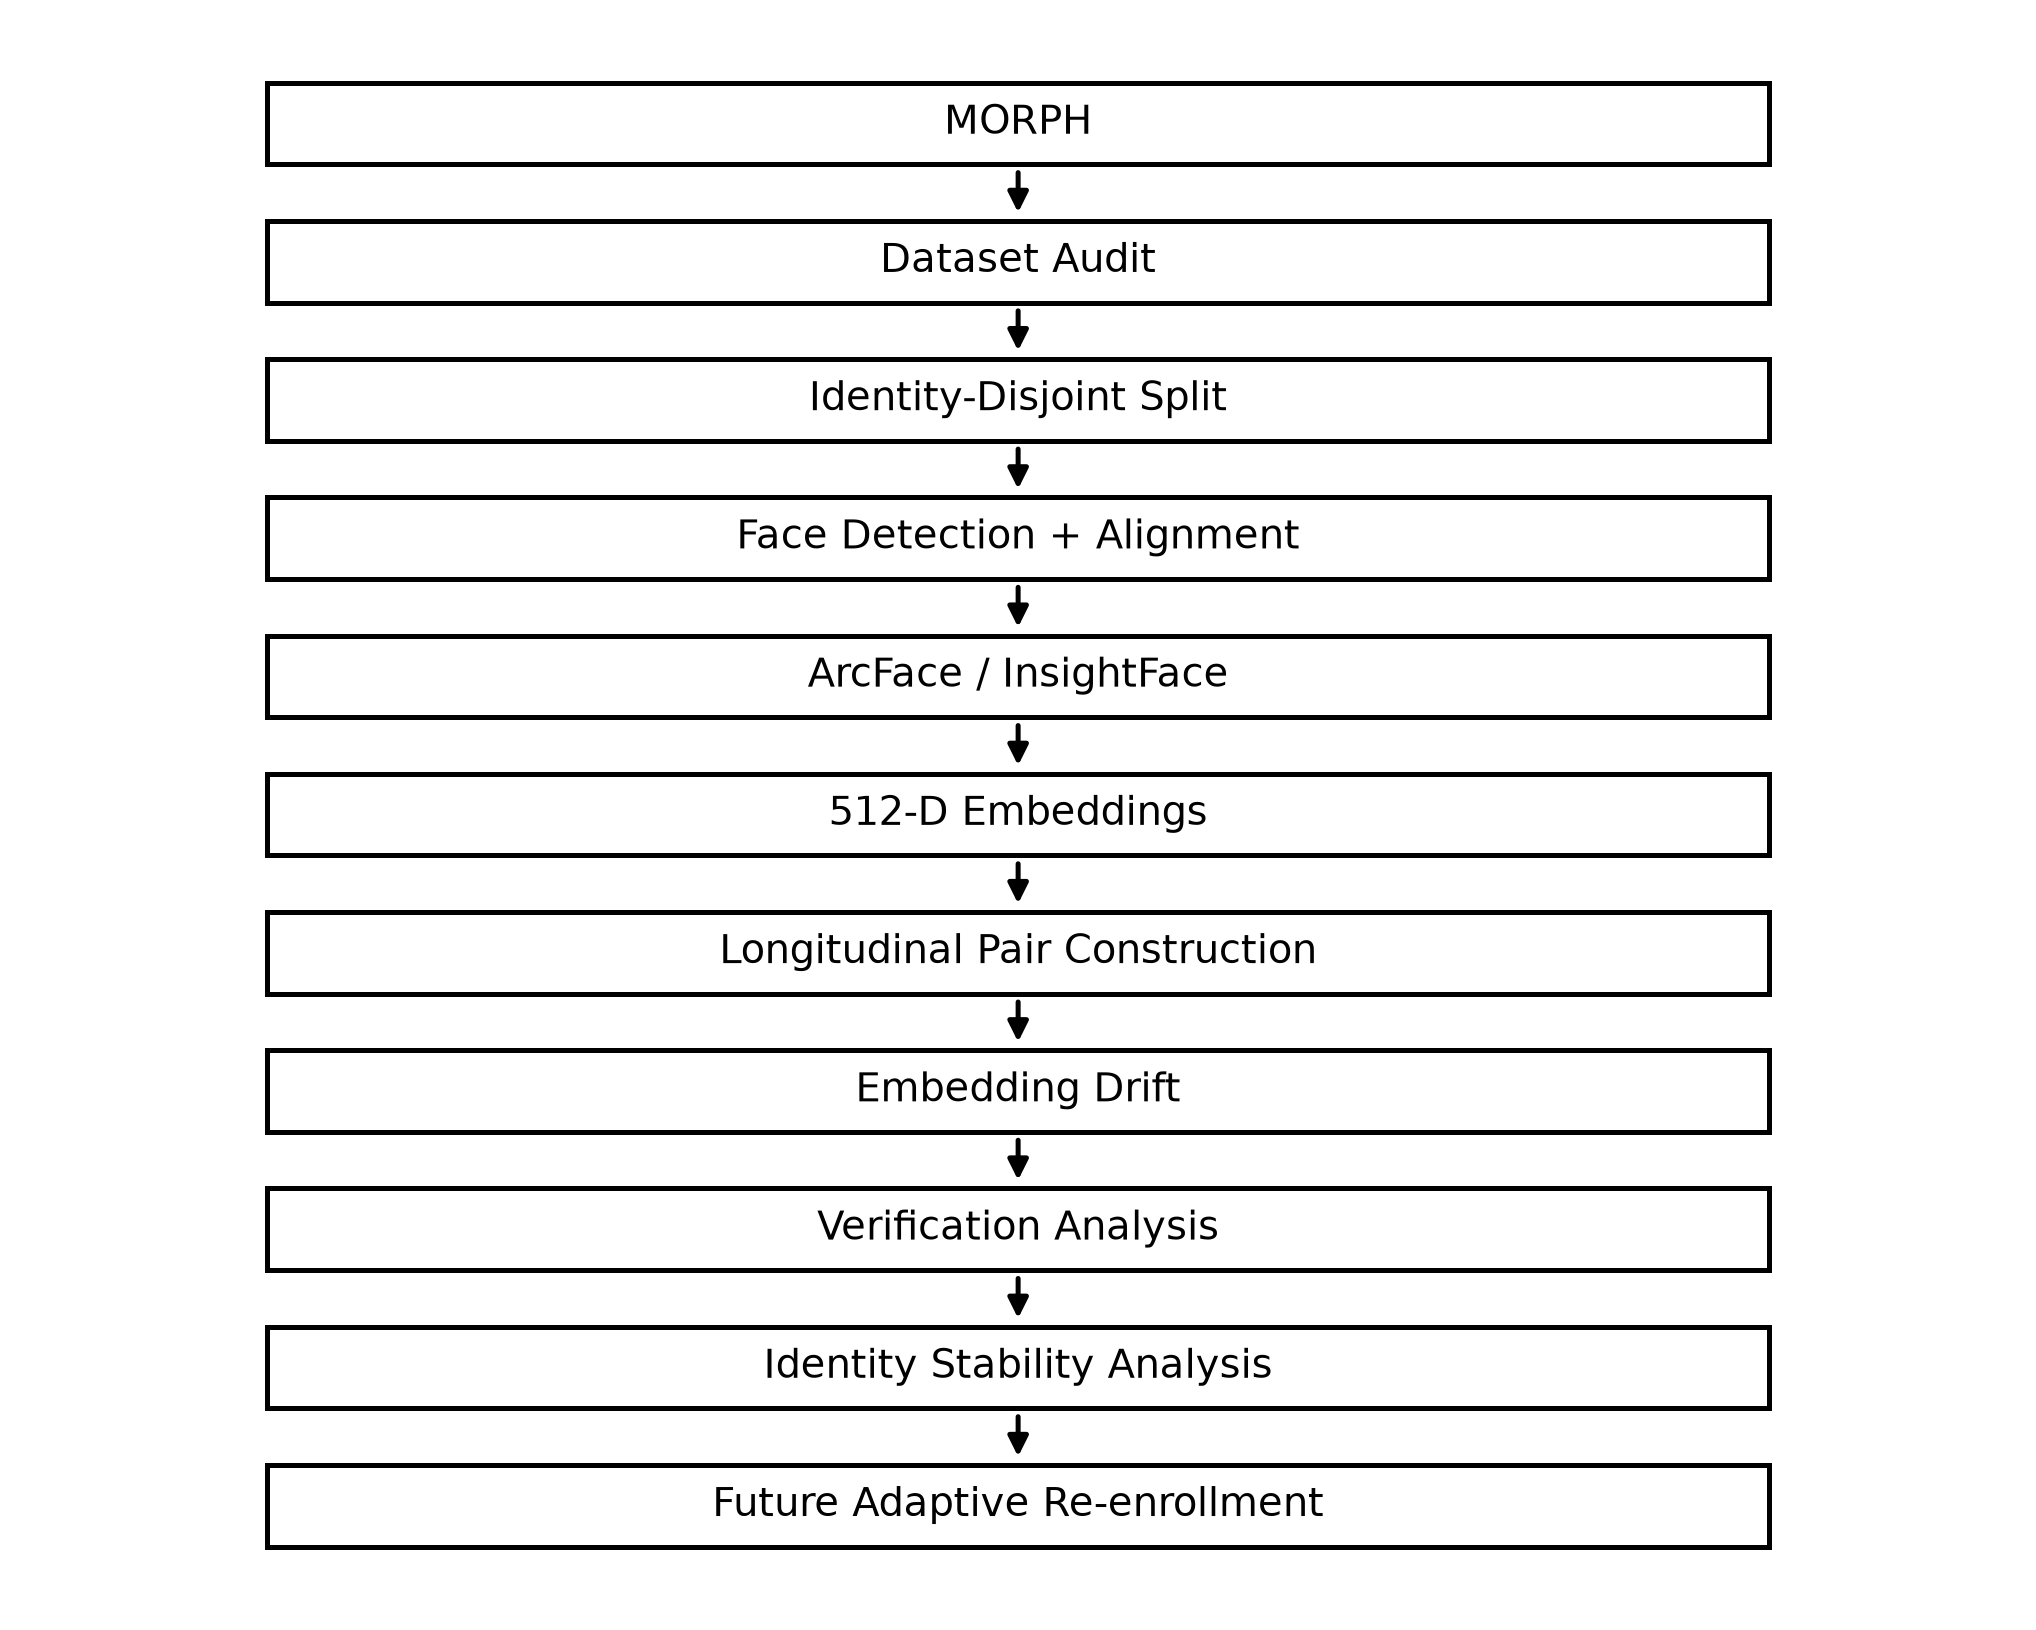
\includegraphics[width=0.95\textwidth]{figures/fig1_pipeline.pdf}
\caption{Research pipeline. The MORPH cohort was audited, split into identity-disjoint train/validation/test subsets, preprocessed, embedded, and analyzed for longitudinal drift and verification behavior. Future adaptive re-enrollment is shown as a future direction rather than a validated contribution.}
\label{fig:pipeline}
\end{figure*}

\begin{figure}[t]
\centering
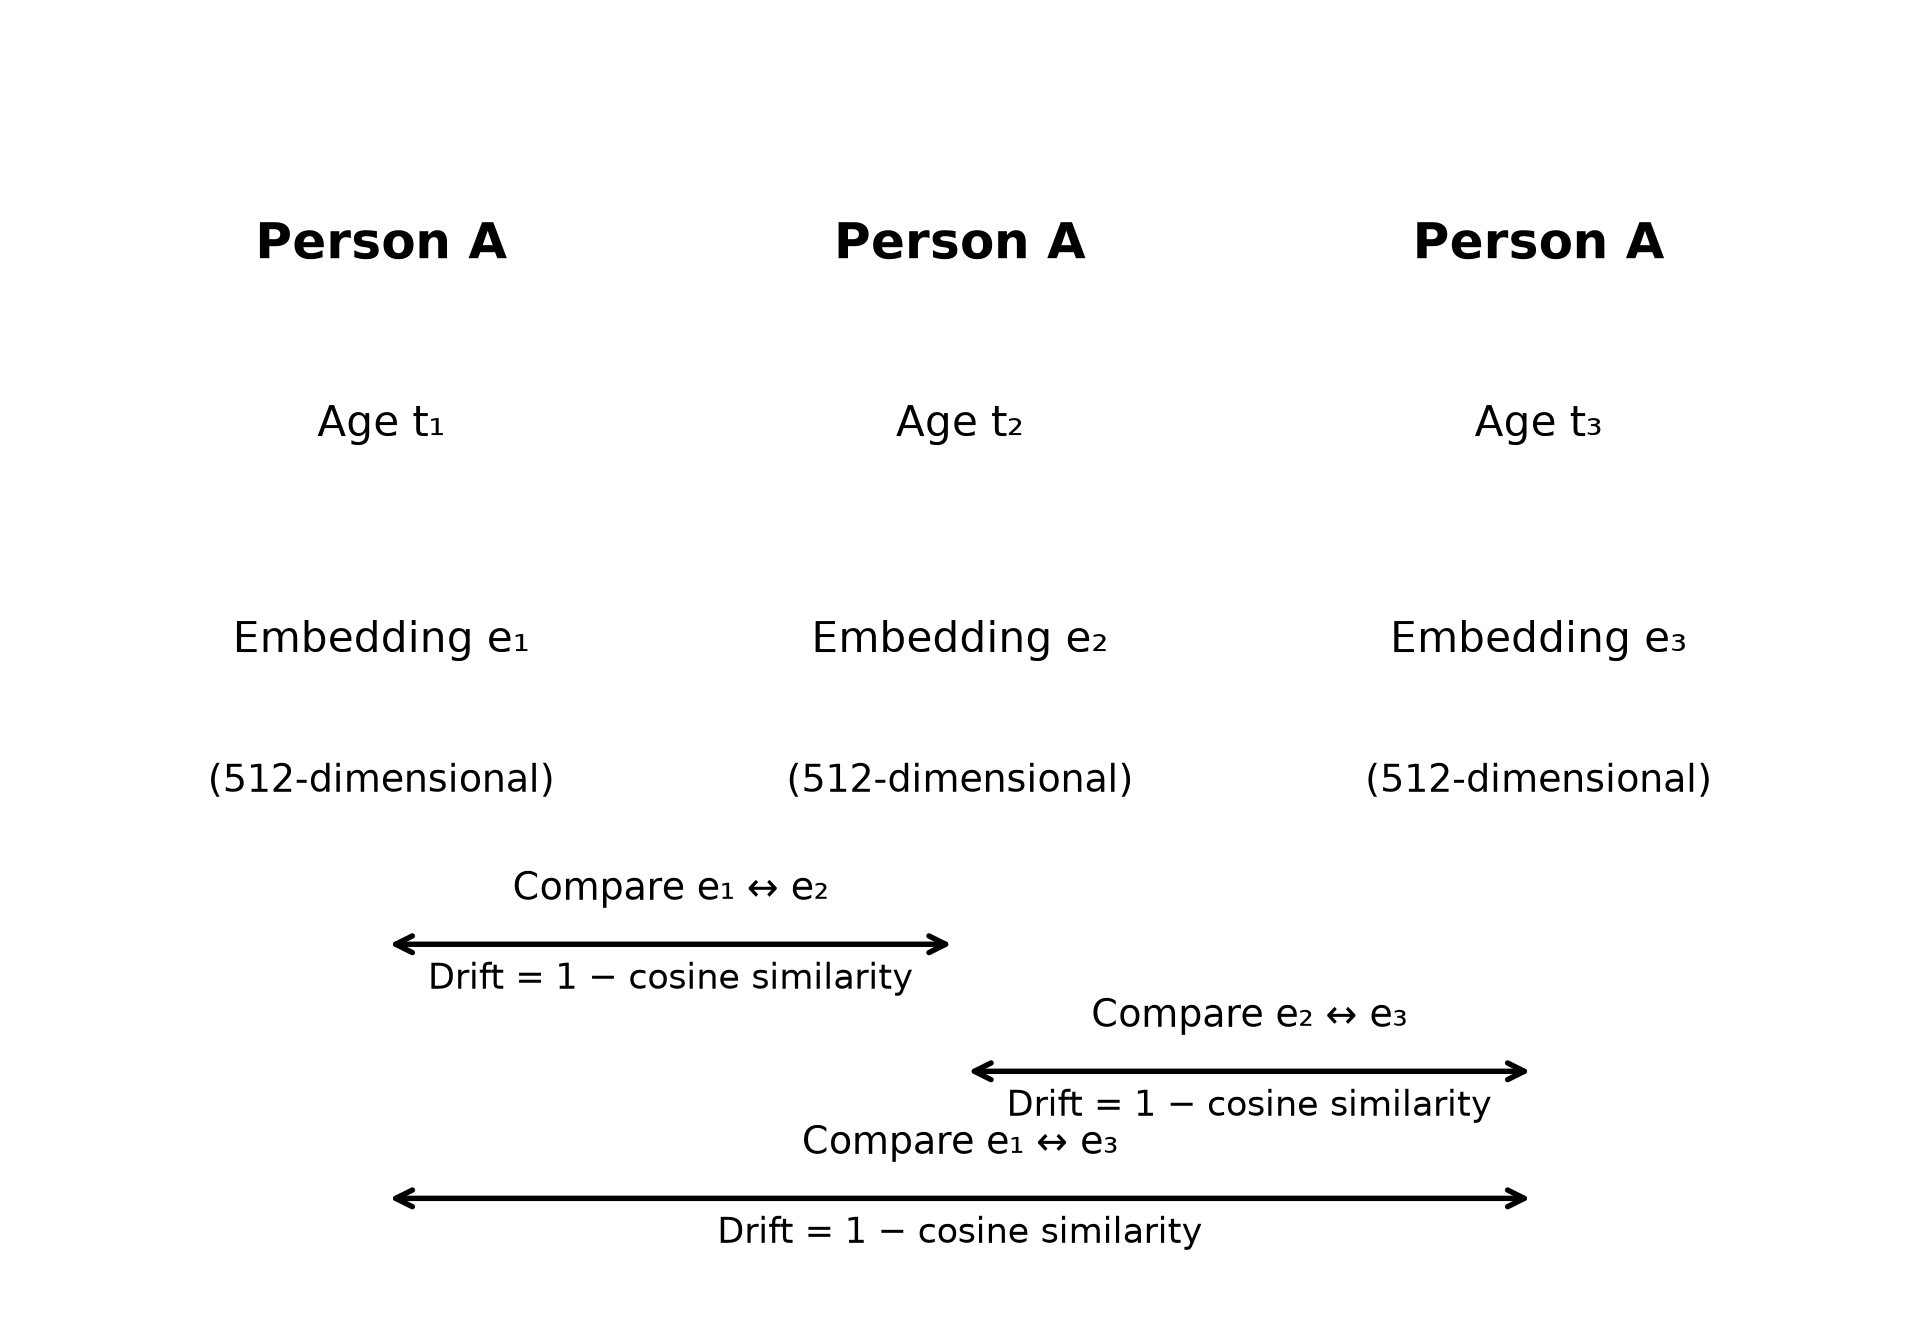
\includegraphics[width=0.85\columnwidth]{figures/fig2_longitudinal_concept.pdf}
\caption{Illustration of longitudinal embedding change. For the same person, observations at ages $t_1$, $t_2$, and $t_3$ produce embeddings $e_1$, $e_2$, and $e_3$. Pairwise cosine similarity and embedding drift are computed for each longitudinal comparison.}
\label{fig:longitudinal_concept}
\end{figure}

\begin{figure}[t]
\centering
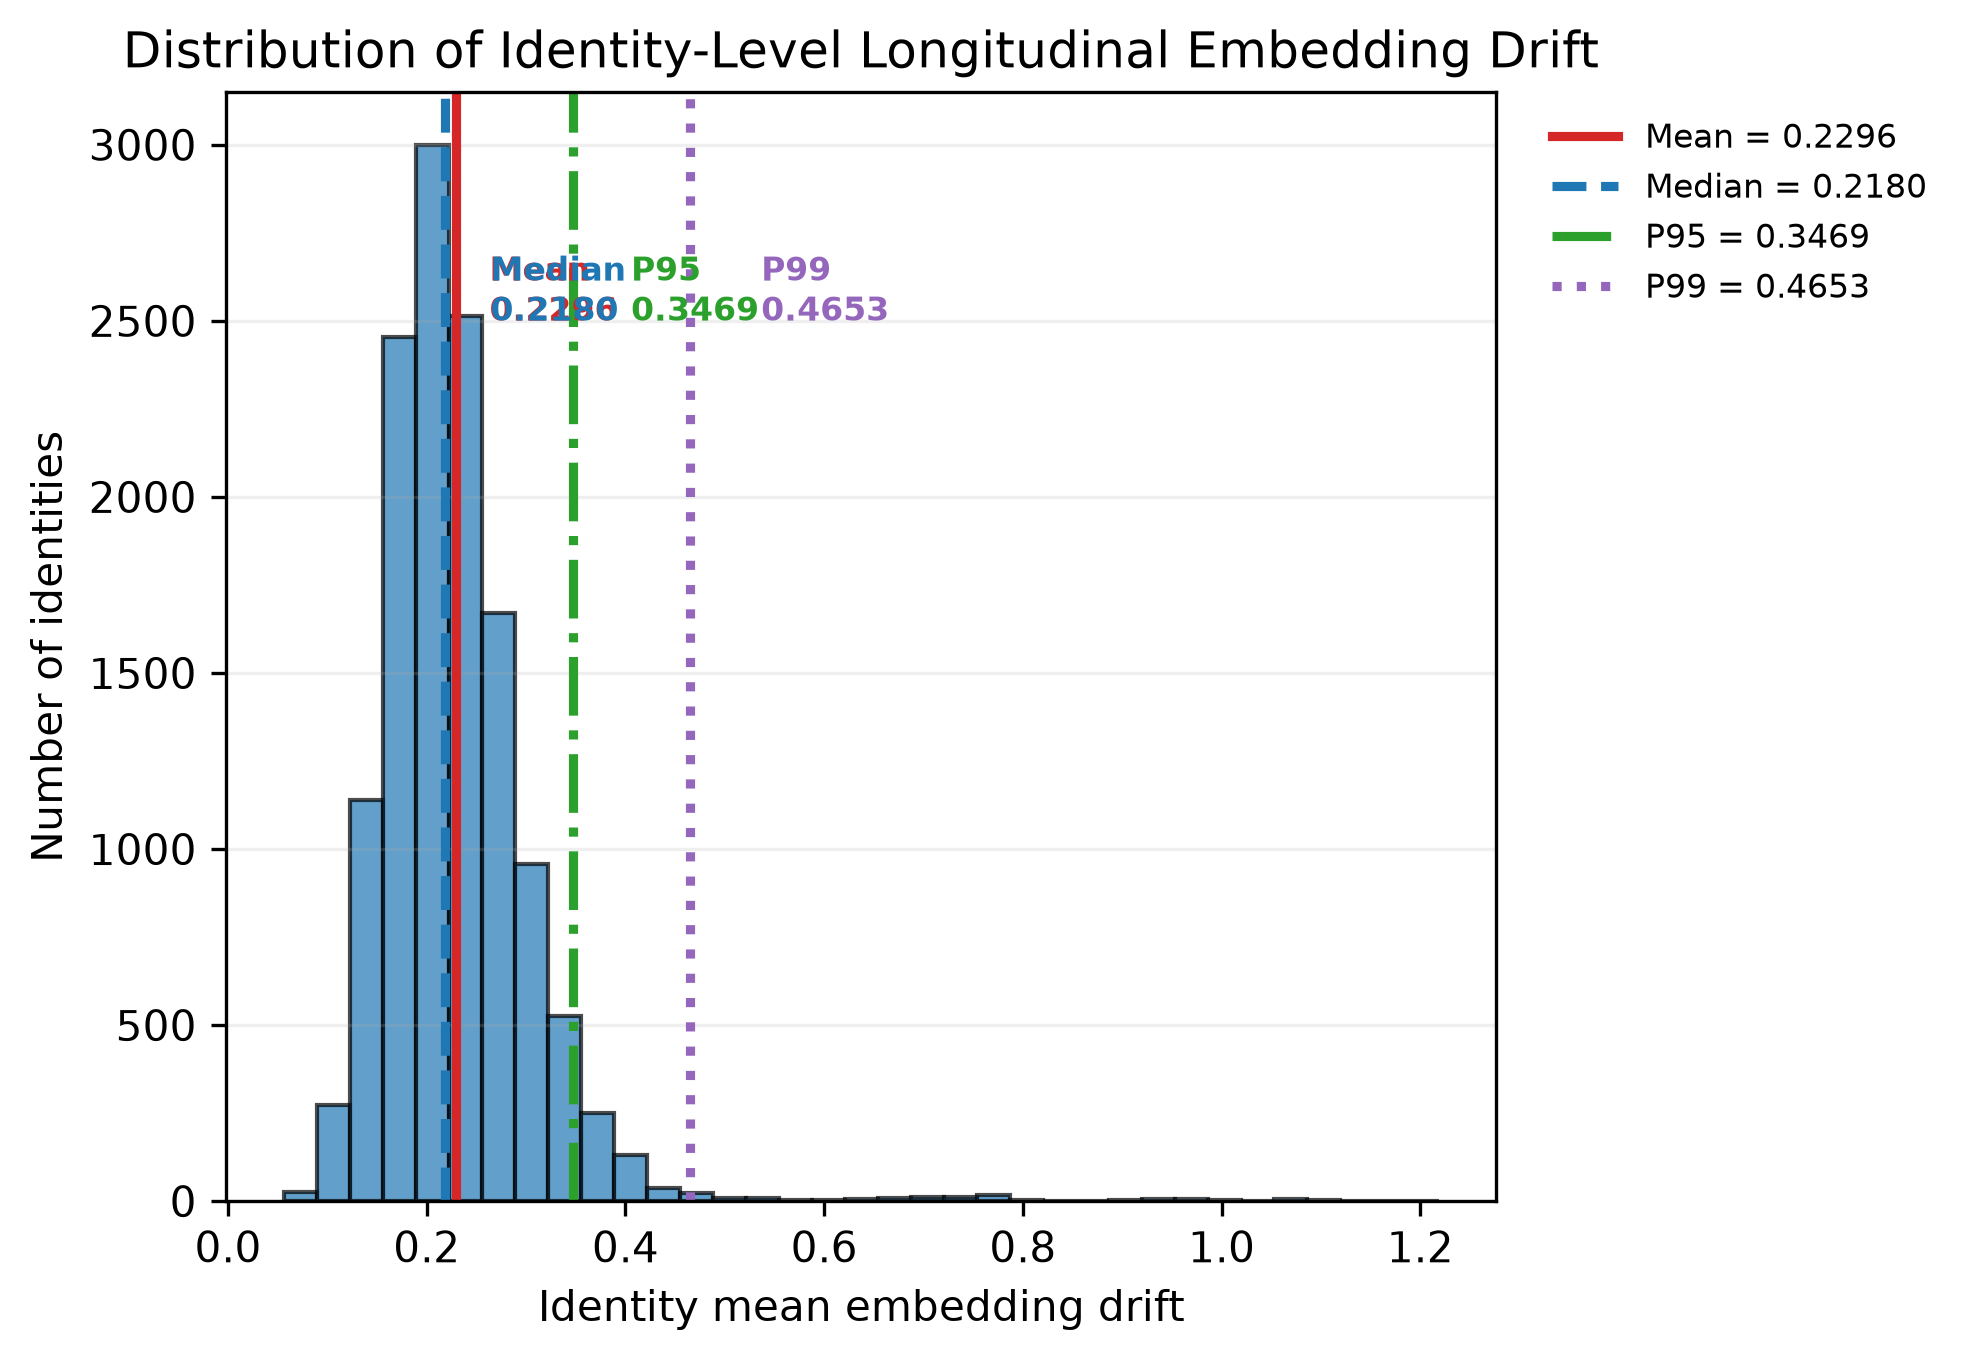
\includegraphics[width=0.9\columnwidth]{figures/fig3_identity_drift_distribution.pdf}
\caption{Identity-level drift distribution across 13,119 identities. The mean is shown with the median, P95, and P99 markers. The distribution is broad and indicates substantial identity heterogeneity in observed representation change.}
\label{fig:identity_drift_distribution}
\end{figure}

\begin{figure}[t]
\centering
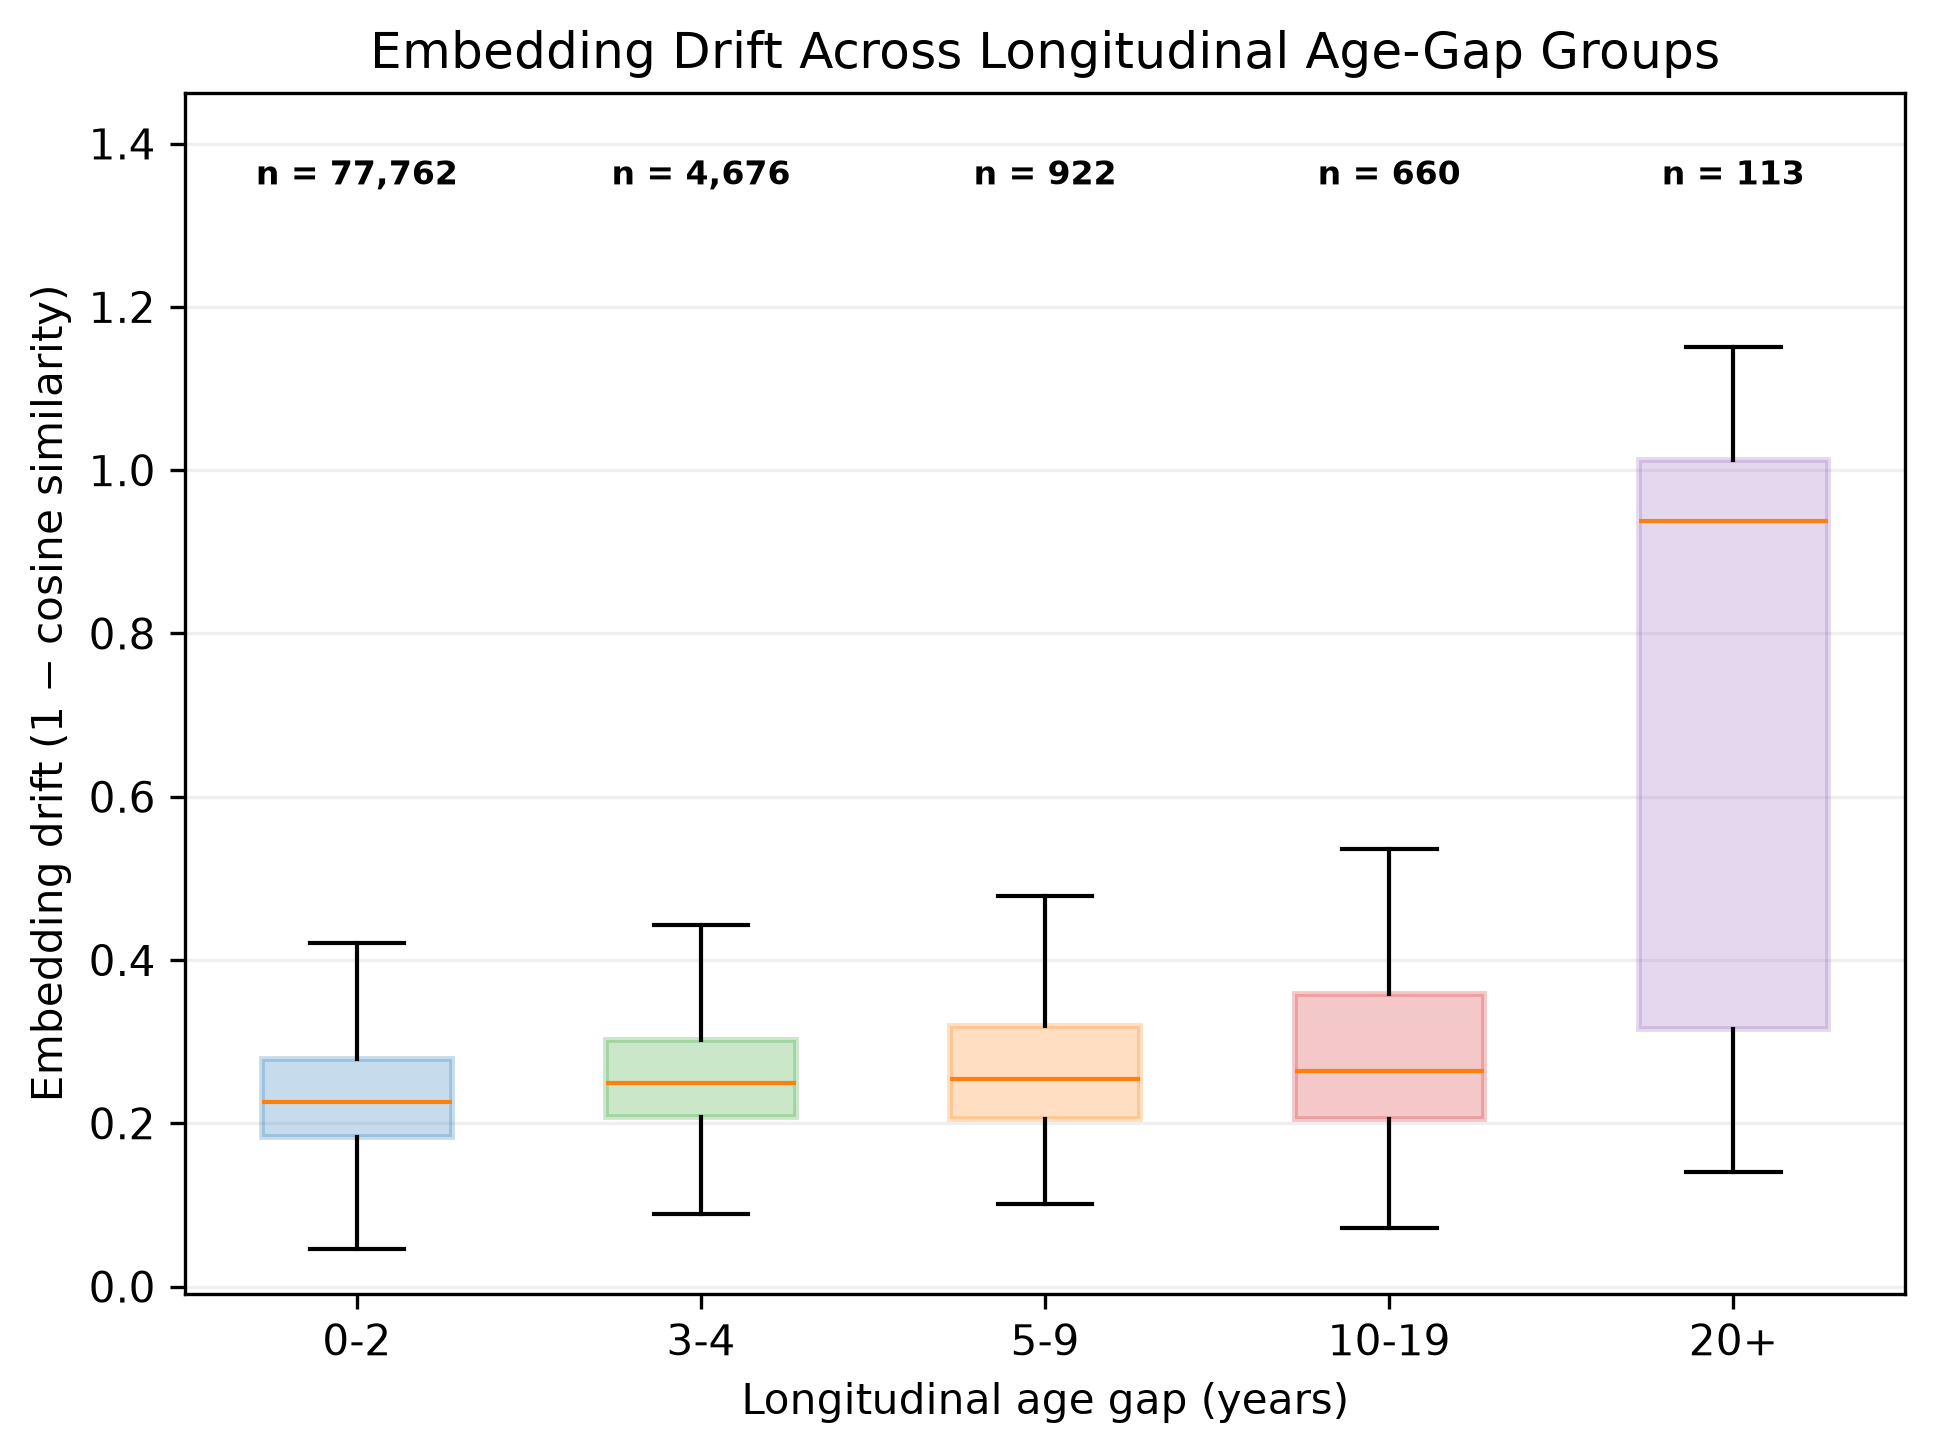
\includegraphics[width=0.9\columnwidth]{figures/fig4_age_gap_drift.pdf}
\caption{Pair-level drift by longitudinal age gap group. Drift increased observedly with age gap in the evaluated MORPH sample. The 20+ year group is shown as an extended-tail case with a limited number of pairs.}
\label{fig:age_gap_drift}
\end{figure}

\begin{figure}[t]
\centering
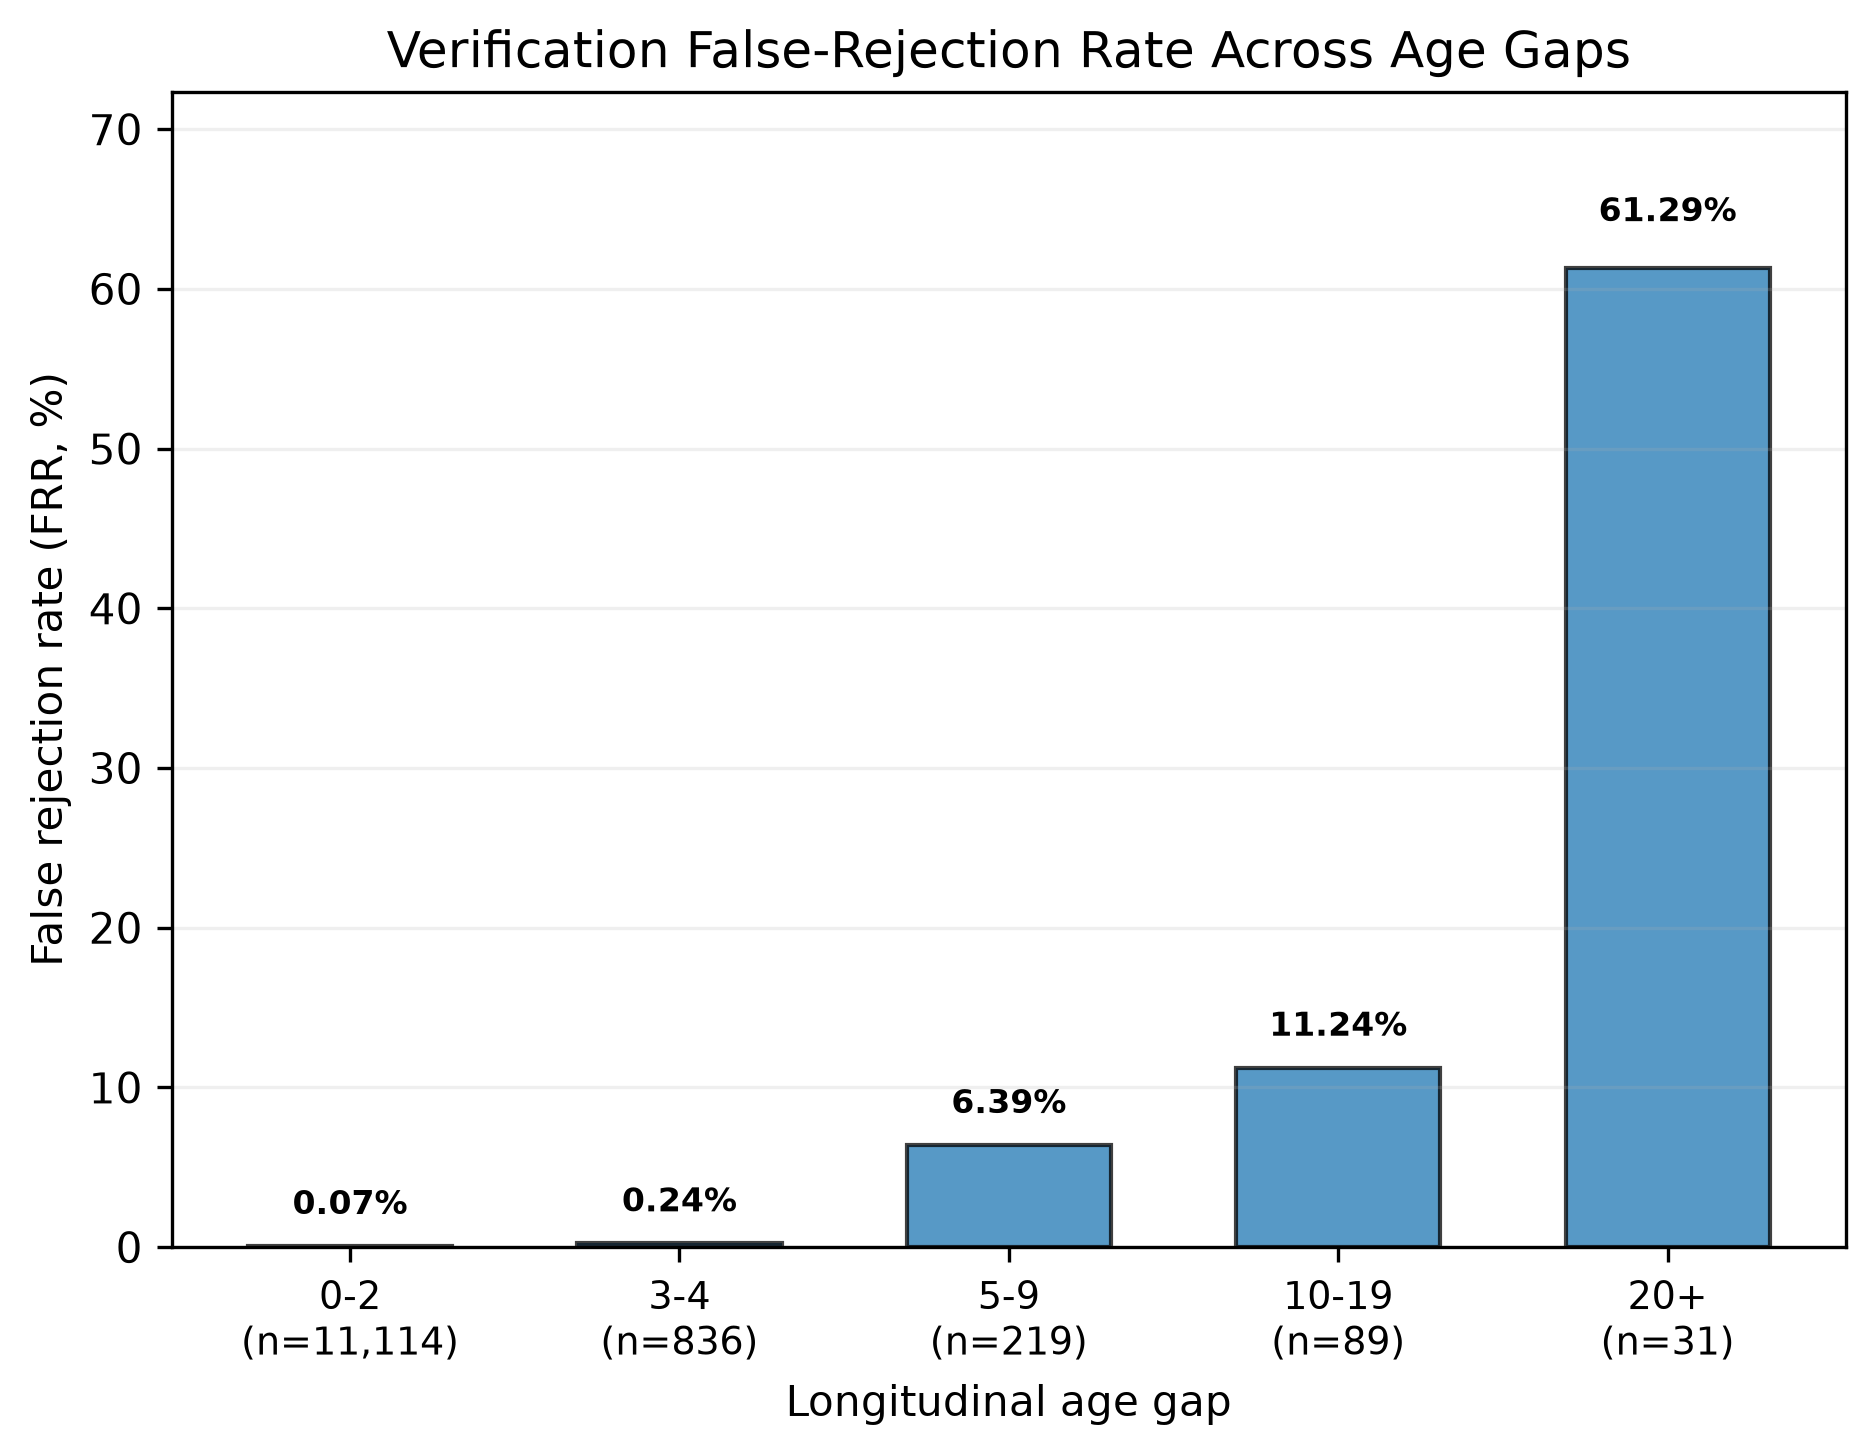
\includegraphics[width=0.9\columnwidth]{figures/fig5_age_gap_verification.pdf}
\caption{Test-set FRR across age-gap groups. Larger longitudinal separation was associated with higher genuine verification failure in this evaluated sample. The 20+ year group contains only 31 pairs.}
\label{fig:age_gap_verification}
\end{figure}

\begin{figure}[t]
\centering
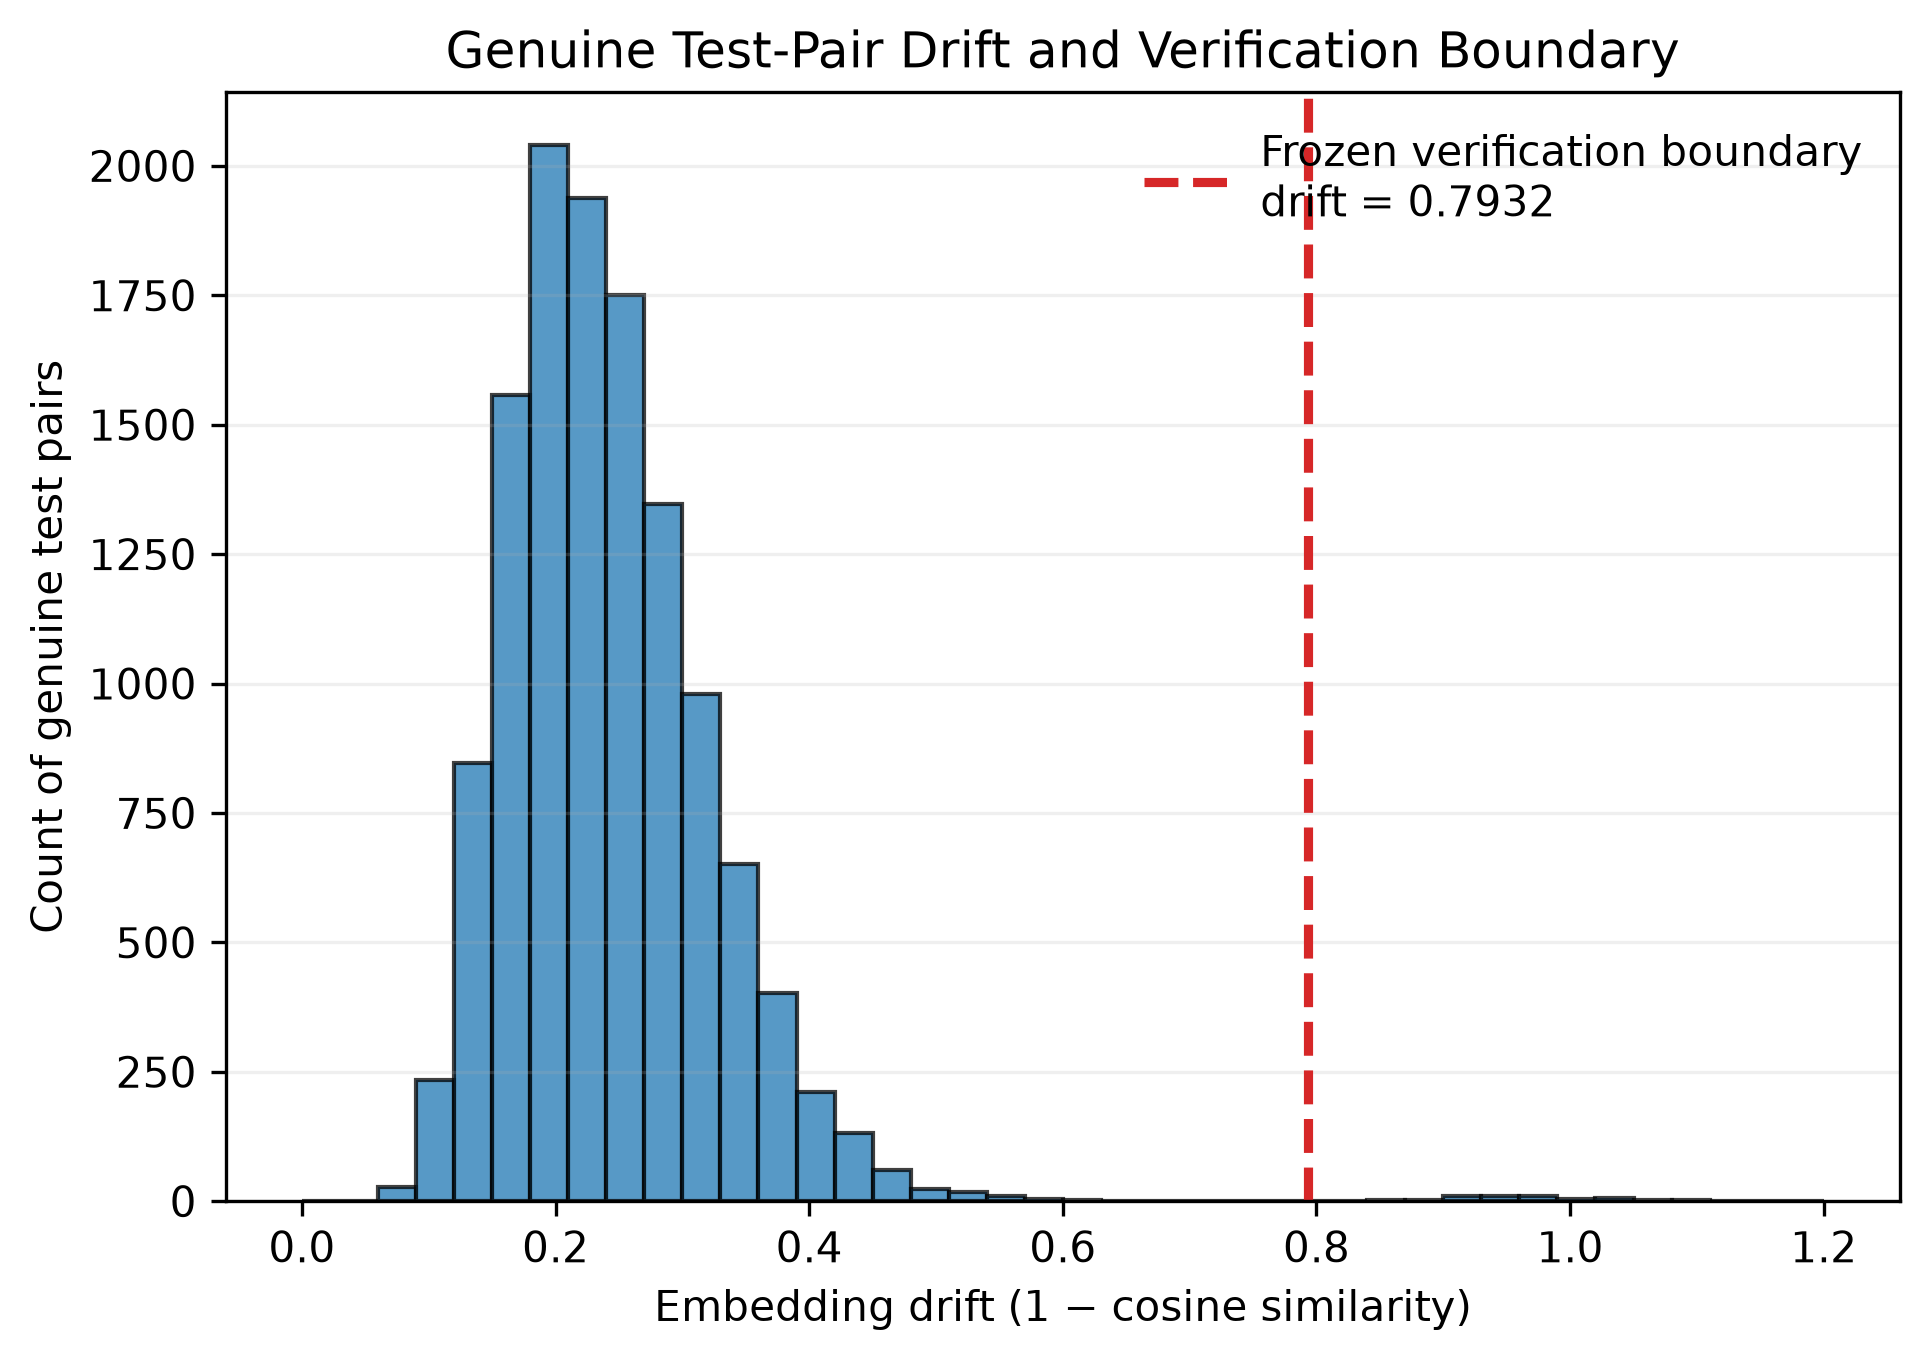
\includegraphics[width=0.9\columnwidth]{figures/fig6_drift_verification_boundary.pdf}
\caption{Observed drift distribution for genuine test pairs and the frozen verification operating boundary at drift $=0.793229669333$. This boundary is a verification operating point, not a validated re-enrollment threshold.}
\label{fig:boundary}
\end{figure}

\begin{figure}[t]
\centering
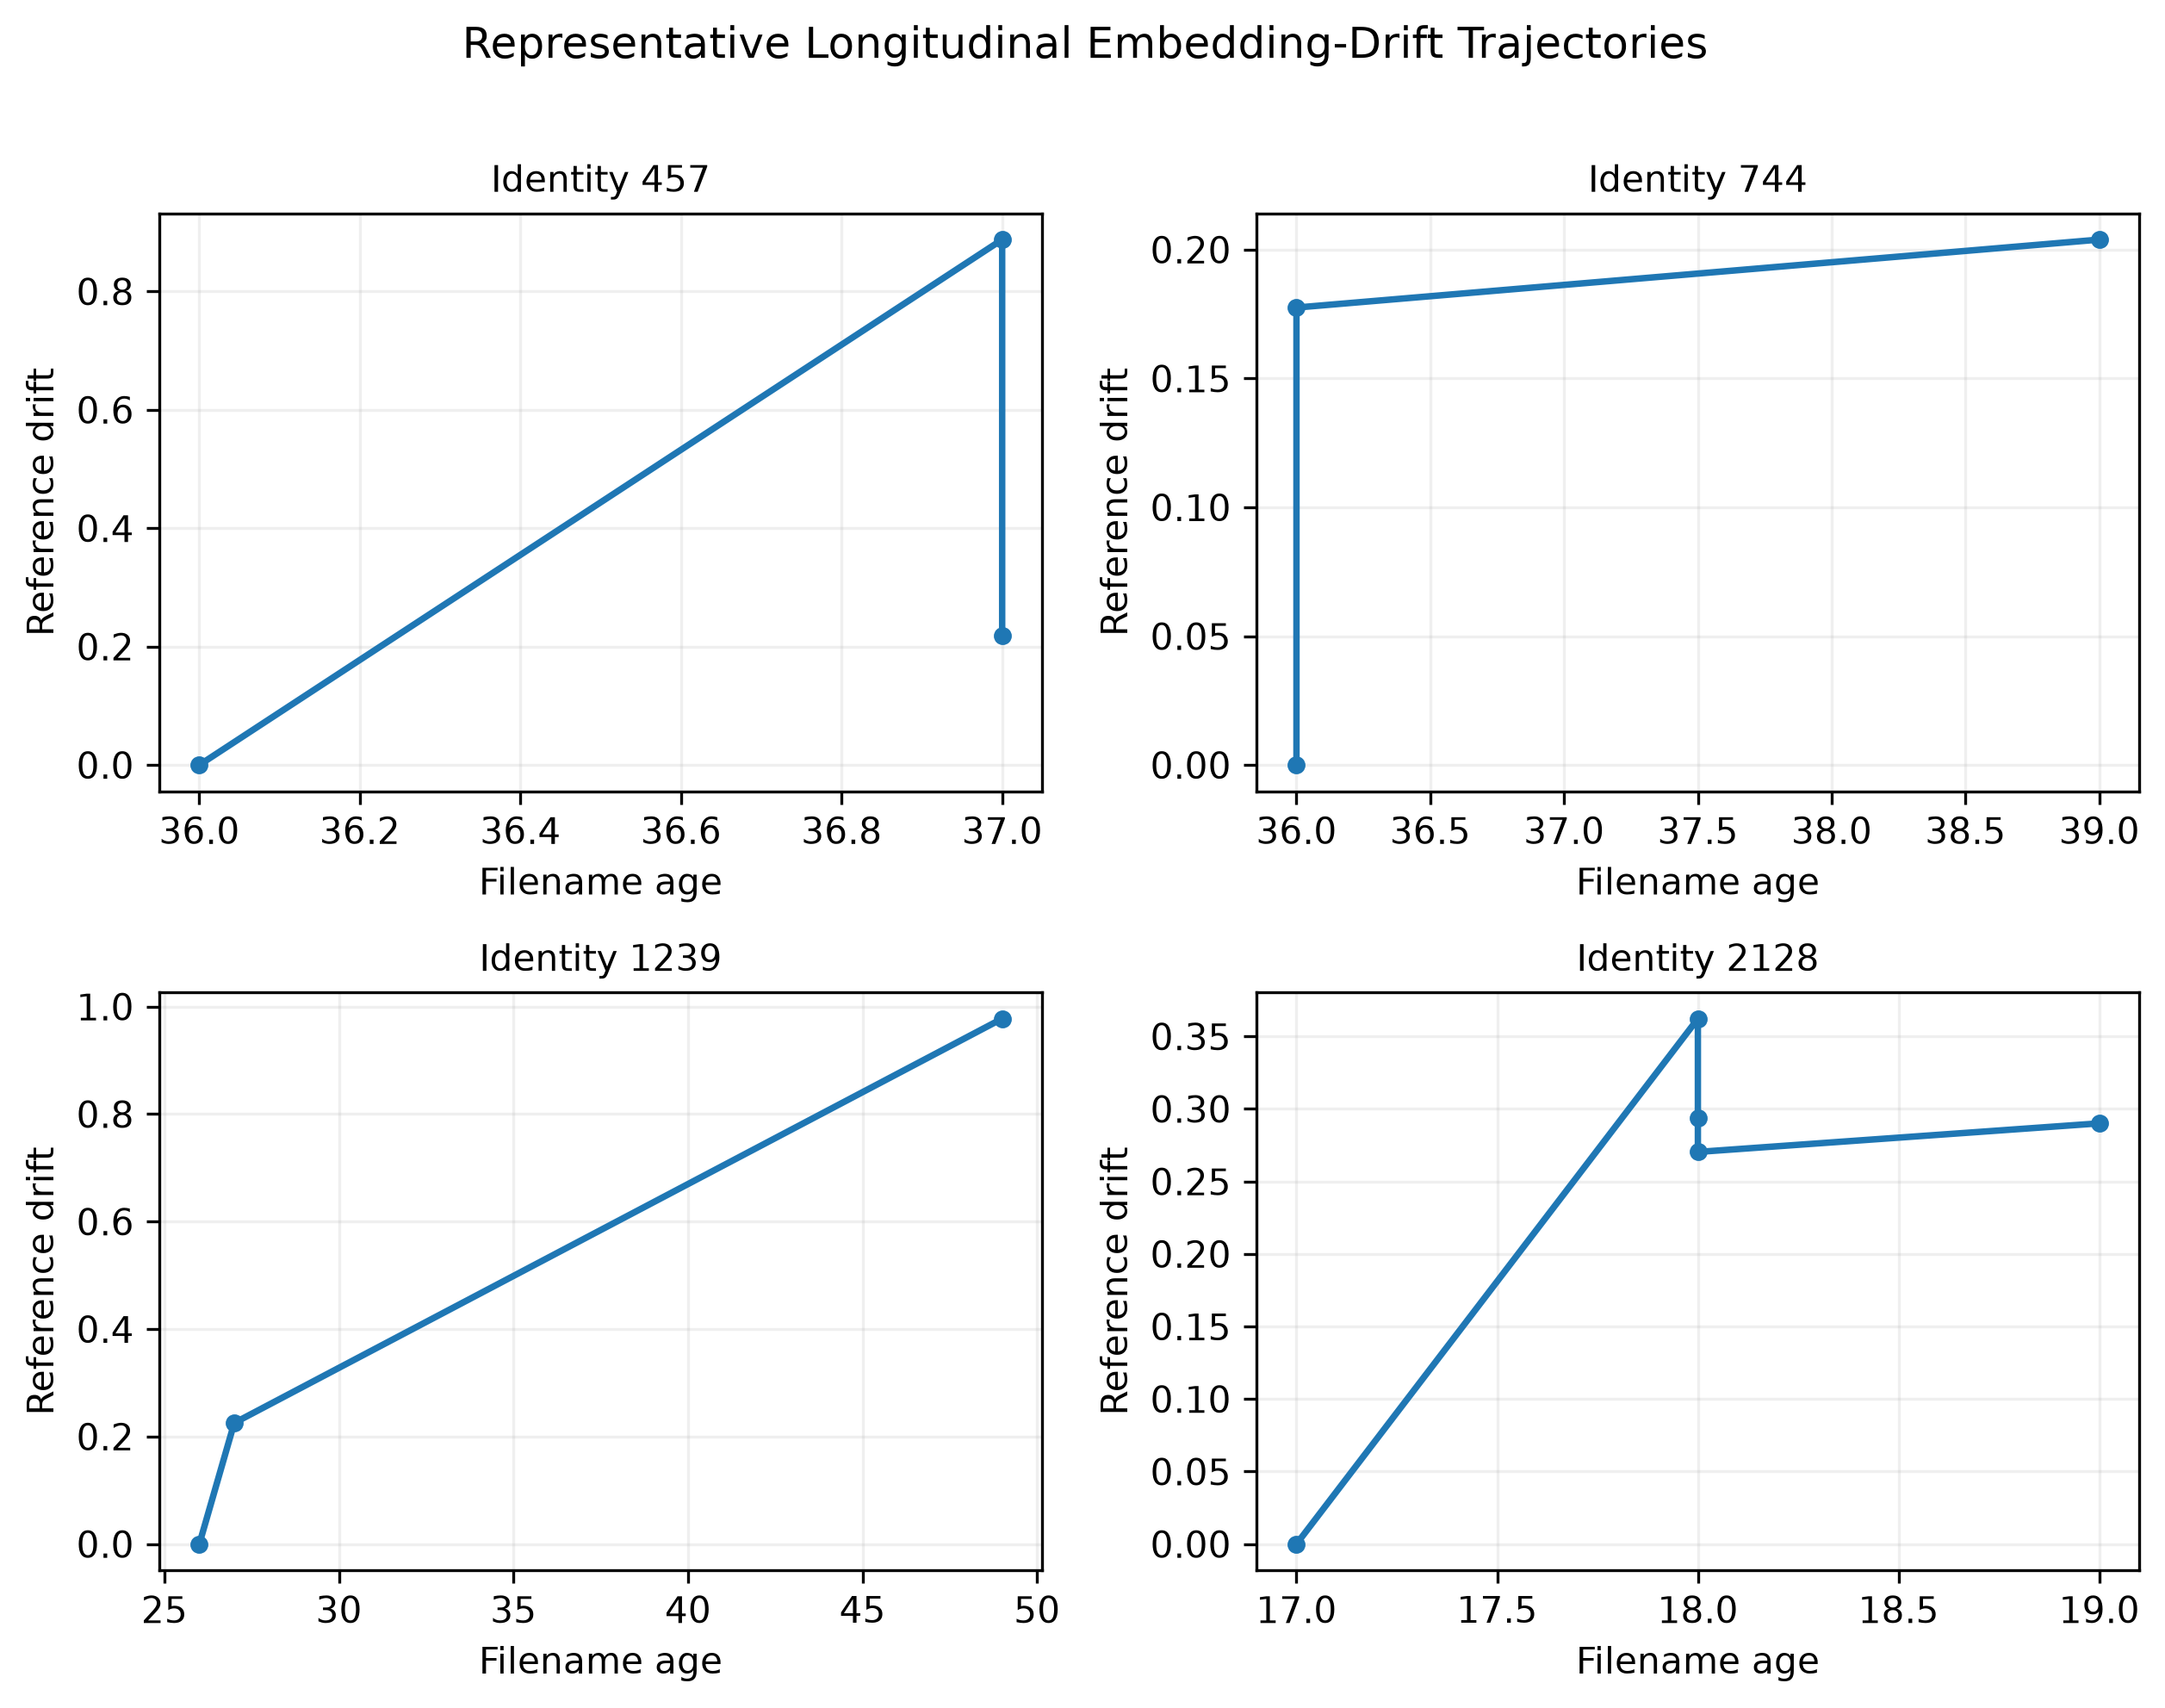
\includegraphics[width=0.9\columnwidth]{figures/fig7_longitudinal_trajectories.pdf}
\caption{Representative longitudinal trajectories from the MORPH data. The examples illustrate stable trajectories, increasing drift, and heterogeneous long-term patterns. These are descriptive identity trajectories; they do not imply a causal mechanism.}
\label{fig:trajectories}
\end{figure}

\bibliographystyle{IEEEtran}
\bibliography{references}

\end{document}
